\begin{enumerate}[font=\bfseries]

    \item \textbf{A video is composed of images that are 512x384 pixels where
    each pixel is 3 bytes or 24 bits. The video is 50 minutes and 40 seconds
    long. Images play at 23 fps. With no compression, how big would this file
    be?}

    \begin{align*}
	\text{Size of Frame} &= 512\text{ pixels}\cdot384\text{
	pixels}\cdot3\text{ bytes} \\
	&= 589824\frac{\text{bytes}}{\text{frame}} \\
	\text{Number of Frames} &=
	\left(50\text{min}\cdot\frac{60\text{s}}{1\text{min}}+40\text{s}\right)
	\cdot23\text{fps} \\
	&= 69920\text{ frames} \\
	\text{Size of File} &= \text{Size of Frame}\cdot
	\text{Number of Frames} \\
	&= 589824\frac{\text{bytes}}{\text{frame}}\cdot69920\text{ frames} \\
	&= 41240494080\text{ bytes}\cdot\frac{1\text{MB}}{2^{20}\text{ bytes}} \\
	&= 39330\text{MB}
    \end{align*}

    \item \textbf{We can treat human fovea as a square sensor array of size
    1.5mmx1.5mm, containing 337,000 cones. Space between cones is equal to the
    width of cones.}
    \begin{enumerate}[label=\alph*., font=\bfseries]
	\item \textbf{What is the field of view in degrees? Assume a focal
	length of 17mm.}

	The fovea is located at one focal length from the lens. Simple
	trigonometry can give us the field of view. We can model this problem as
	an isosceles triangle. $\theta$ is the field of view, n is the fovea
	height, and m is the focal length.

	\begin{align*}
	    \tan\left(\frac{\theta}{2}\right) &= \frac{n}{2m} \\
	    \tan^{-1}\left(\frac{n}{2m}\right) &= \frac{\theta}{2} \\
	    \theta &= 2\tan^{-1}\left(\frac{n}{2m}\right) \\
	    \theta &= 2\tan^{-1}\left(\frac{1.5\text{mm}}{2\cdot17\text{mm}}\right) \\
	    \theta &= 5.05^{\circ} 
	\end{align*}

\pagebreak

	\item \textbf{A person obvserves a fishing boat out at sea that is
	approximately 1 mile away. The person claims that they can see a seagull
	following the boat. Is that possible? Justify your answer with
	quantitative estimates. Assume for simplicity that the size of the image
	of the seagull must cover two receptors. Seagulls can range in size from
	29cm to 76cm.}

	First we need to determine the height of a cone:

	\begin{align*}
	    h &= \frac{1.5\text{mm}}{\sqrt{33700}} \\
	    &= 2.58\mu\text{m}
	\end{align*}

	We know that there are 337,000 cones in the fovea, and that we are
	treating it as a square. The height of a cone can be found dividing the
	height of the fovea by the square root of the total number of cones. We
	can find the image height of a seagull through scaling laws of
	triangles. This gives us:

	\begin{align*}
	    \text{Image Height} &= \text{Seagull
	    Height}\cdot\frac{17\text{mm}}{1\text{ mile}}
	\end{align*}

	This gives us the results:

	\begin{align*}
	    \text{Small Seagull Image Height} &= 3.06\mu\text{m}\\
	    \text{Large Seagull Image Height} &= 8.03\mu\text{m}
	\end{align*}

	We can see that a small seagull would be detected by only one cone,
	where we need two cones to detect the seagull. A large seagull registers
	as 3 cones, therefore the person may be telling the truth.

    \end{enumerate}

\pagebreak

    \item \textbf{It is often useful to generate a synthetic image with known
    properties that can be used to test algorithms. Generate an image composed
    of two concentric circles as shown below. The inner circle should have a
    radius of 50 pixels and a mean value of 192. The outer circle should have a
    radius of 100 pixels and a mean value of 128. The background should have a
    value of 64. Add a uniform random noise to each pixel in the range of -16 to
    16. Save the image in tif format,and make sure the saved image looks
    correct.}
    
    To play around with some other image processing tools, I used the CImg
    library to generate this image:

    \begin{figure}[H]
	\centering
	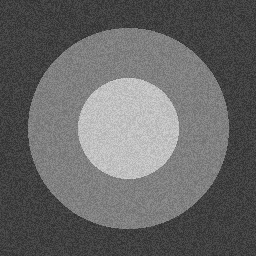
\includegraphics{testImage.png}
    \end{figure}
   
\pagebreak

    CImg is a C++ library for image processing. It is very portable and can
    compile down to very efficient object code. I used the C++11 random header
    functions to generate the noise in the image.

    \lstinputlisting[language=c++, basicstyle=\small]{../q3/main.cpp}

\pagebreak

    \item \textbf{You are given one image f1. You are asked to synthesize an
    image f2 that is f1 shifted 5 pixels to the right, 2 pixels up, and then
    rotated by 30 degrees clockwise. Assume f1 uses image coordinates (x,y) and
    f1 uses image coordinates (u,v).}
    \begin{enumerate}[label=\alph*., font=\bfseries]
	\item \textbf{Find the forward mapping function from f1 to f2.}

	Forward mapping can simply be defined as:

	$$ f2 = f1 \times T$$
	
	And a transformation can be broken down to simple parts. In our case we
	have two different transformations, shifting and rotation. The shifting
	transform is: 
	
	$$
	\begin{bmatrix}
	1 & 0 & 0 \\
	0 & 1 & 0 \\
	5 & -2 & 1
	\end{bmatrix} 
	$$
	
	and the rotation transform is:
	
	$$
	\begin{bmatrix}
	\cos30^\circ & \sin30^\circ & 0 \\
	-\sin30^\circ & \cos30^\circ\ & 0 \\
	0 & 0 & 1 
	\end{bmatrix}
	$$
	
	Multiplying those together gets our full transformation function:

	$$
	\begin{bmatrix}
	\cos30^\circ & \sin30^\circ & 0 \\
	-\sin30^\circ & \cos30^\circ\ & 0 \\
	5 & -2 & 1 
	\end{bmatrix}
	$$
	
	\item \textbf{Find the inverse mapping function f2 to f1.}

	The inverse mapping function is actually just the inverse of the forward
	mapping transform matrix. This gives us: 

	$$
	\begin{bmatrix}
	\cos30^\circ & \sin30^\circ & 2\sin30^\circ - 5\cos30^\circ \\
	-\sin30^\circ & \cos30^\circ & 5\sin30^\circ + 2\cos30^\circ \\
	0 & 0 & 1
	\end{bmatrix}
	$$

	\item \textbf{How can you generate f2 using step (a) or (b)?}
	
	When you are forward mapping an image, each pixel is transformed onto
	the second image. Once that is done, any pixels that did not recieve a
	value in the second image must be assigned some value. Additionally,
	further complexities occur when multiple pixel values in the first image
	want to be written to a single pixel in the second image. \\

	In the inverse mapping mathod we apply the inverse mapping transform to
	an empty second image. We go from pixel to pixel in this image and find
	where it "exists" in the original image. This can give us a position
	that is between actual pixel locations and in this case we use an
	interpolation method to determine its actual value. This method
	naturally deals with "collisions" and out of bound pixels are detected
	easily.

    \end{enumerate}

\end{enumerate}
